\documentclass{beamer}
\usepackage[utf8]{inputenc}

\usetheme{Boadilla}
\usecolortheme{lily}
\usepackage{amsmath,amssymb,amsfonts,amsthm}
\usepackage{mathtools}
\usepackage{txfonts}
\usepackage{tkz-euclide}
\usepackage{listings}
\usepackage{adjustbox}
\usepackage{array}
\usepackage{tabularx}
\usepackage{lmodern}
\usepackage{gvv}
\usepackage{circuitikz}
\usepackage{tikz}
\usepackage{graphicx}

\setbeamertemplate{footline}
{
  \leavevmode%
  \hbox{%
  \begin{beamercolorbox}[wd=\paperwidth,ht=2.25ex,dp=1ex,right]{author in head/foot}%
    \insertframenumber{} / \inserttotalframenumber\hspace*{2ex} 
  \end{beamercolorbox}}%
  \vskip0pt%
}

\usepackage{tcolorbox}
\tcbuselibrary{minted,breakable,xparse,skins}




\providecommand{\nCr}[2]{\,^{#1}C_{#2}} % nCr
\providecommand{\nPr}[2]{\,^{#1}P_{#2}} % nPr
\providecommand{\mbf}{\mathbf}
\providecommand{\pr}[1]{\ensuremath{\Pr\left(#1\right)}}
\providecommand{\qfunc}[1]{\ensuremath{Q\left(#1\right)}}
\providecommand{\sbrak}[1]{\ensuremath{{}\left[#1\right]}}
\providecommand{\lsbrak}[1]{\ensuremath{{}\left[#1\right.}}
\providecommand{\rsbrak}[1]{\ensuremath{{}\left.#1\right]}}
\providecommand{\brak}[1]{\ensuremath{\left(#1\right)}}
\providecommand{\lbrak}[1]{\ensuremath{\left(#1\right.}}
\providecommand{\rbrak}[1]{\ensuremath{\left.#1\right)}}
\providecommand{\cbrak}[1]{\ensuremath{\left\{#1\right\}}}
\providecommand{\lcbrak}[1]{\ensuremath{\left\{#1\right.}}
\providecommand{\rcbrak}[1]{\ensuremath{\left.#1\right\}}}
\theoremstyle{remark}
\newcommand{\sgn}{\mathop{\mathrm{sgn}}}
\providecommand{\abs}[1]{\left\vert#1\right\vert}
\providecommand{\res}[1]{\Res\displaylimits_{#1}} 
\providecommand{\norm}[1]{\lVert#1\rVert}
\providecommand{\mtx}[1]{\mathbf{#1}}
\providecommand{\mean}[1]{E\left[ #1 \right]}
\providecommand{\fourier}{\overset{\mathcal{F}}{ \rightleftharpoons}}
%\providecommand{\hilbert}{\overset{\mathcal{H}}{ \rightleftharpoons}}
\providecommand{\system}{\overset{\mathcal{H}}{ \longleftrightarrow}}
	%\newcommand{\solution}[2]{\textbf{Solution:}{#1}}
%\newcommand{\solution}{\noindent \textbf{Solution: }}
\providecommand{\dec}[2]{\ensuremath{\overset{#1}{\underset{#2}{\gtrless}}}}
\newcommand{\myvec}[1]{\ensuremath{\begin{pmatrix}#1\end{pmatrix}}}
\let\vec\mathbf

\lstset{
%language=C,
frame=single, 
breaklines=true,
columns=fullflexible
}

\numberwithin{equation}{section}

\lstset{
  language=Python,
  basicstyle=\ttfamily\small,
  keywordstyle=\color{blue},
  stringstyle=\color{orange},
  numbers=left,
  numberstyle=\tiny\color{gray},
  breaklines=true,
  showstringspaces=false
}

\title{Problem 7.4.30}
\author{ee25btech11023-Venkata Sai}

\date{\today} 
\begin{document}

\begin{frame}
\titlepage
\end{frame}

\section*{Outline}
\begin{frame}
\tableofcontents
\end{frame}

\section{Problem}

\begin{frame}
\frametitle{Problem}
A circle is given by $x^2+(y - 1)^2=1$, another circle C touches it externally and also the $X$ axis, then the locus of its centre is \\
\begin{enumerate}
\item$ \cbrak{\brak{x,y}:x^2=4y} \bigcup \cbrak{\brak{x,y}:y\leq0}$
\item  $ \cbrak{\brak{x,y}:x^2+\brak{y-1}^2 = 4} \bigcup \cbrak{\brak{x,y}:y\leq0} $
\item  $\cbrak{\brak{x,y}:x^2=4y} \bigcup \cbrak{\brak{0,y}:y\leq0}$   
\item $ \cbrak{\brak{x,y}:x^2=4y} \bigcup \cbrak{\brak{0,y}:y\leq0}$
\end{enumerate}
\end{frame}
%\subsection{Literature}
\section{Solution}

\subsection{Formula}
\setcounter{section}{1}
\begin{frame}
\frametitle{Formula}
As the circle touches $X-$axis , Distance of a point from $x$-axis is given by
\begin{align}
    r=|\vec{n}^\top\vec{c}|
\end{align}
where $\vec{n}$ is the unit vector normal to $x$-axis\\
For the given circle with radius $r_1$ and center $c_1$
\begin{align}
 x^2+(y - 1)^2=1\\
 \vec{p}=\myvec{0\\1}=\vec{n}\ \text{and}\ r_1=1 
\end{align}
Distance between their centers equal to sum of their radius
\begin{align}
    \norm{\vec{c}-\vec{p}}&=r+r_1\\
\norm{\vec{c}-\vec{n}}&=|\vec{n}^\top\vec{c}|+1 \\
\norm{\vec{c}-\vec{n}}^2&=\brak{|\vec{n}^\top\vec{c}|+1}^2 
\end{align}
\end{frame}
\subsection{Squaring}
\begin{frame}
\frametitle{Squaring}
\begin{align}
\brak{\vec{c}-\vec{n}}\brak{\vec{c}^\top-\vec{n}^\top}=\brak{|\vec{n}^\top\vec{c}|+1}^2 
\end{align}
\begin{align}
\vec{c}^\top\vec{c}+\vec{n}\vec{n}^\top-\vec{c}^\top\vec{n}-\vec{n}^\top\vec{c}&= \brak{|\vec{n}^\top\vec{c}|}^2+2|\vec{n}^\top\vec{c}|+1\\
\vec{c}^\top\vec{c}+\vec{n}\vec{n}^\top-\vec{c}^\top\vec{n}-\vec{n}^\top\vec{c}&=\brak{\vec{n}^\top\vec{c}}^\top\brak{\vec{n}^\top\vec{c}}+2|\vec{n}^\top\vec{c}|+1\\
\vec{c}^\top\vec{c}+\norm{\vec{n}}^2-2\vec{n}^\top\vec{c}&=\brak{\vec{c}^\top\vec{n}\vec{n}^\top\vec{c}}+2|\vec{n}^\top\vec{c}|+1 
\end{align}
\begin{align}
\vec{c}^\top\vec{c}+1&=\brak{\vec{c}^\top\vec{n}\vec{n}^\top\vec{c}}+2\vec{n}^\top\vec{c}+2|\vec{n}^\top\vec{c}|+1 
\end{align}
\begin{align}
\vec{c}^\top\vec{c}-\brak{\vec{c}^\top\vec{n}\vec{n}^\top\vec{c}}=2\vec{n}^\top\vec{c}+2|\vec{n}^\top\vec{c}| \\
\vec{c}^\top\brak{\vec{I}-\vec{n}\vec{n}^\top}\vec{c}=2\vec{n}^\top\vec{c}+2|\vec{n}^\top\vec{c}| 
\end{align}
\end{frame}
\subsection{Outer Product}
\begin{frame}
\frametitle{Outer Product}
\begin{align}
\vec{c}^\top\brak{\myvec{1&0\\0&1}-\myvec{0\\1}\myvec{0&1}}\vec{c}=2\myvec{0\\1}^\top\vec{c}+2\left|\myvec{0\\1}^\top\vec{c}\right| \\
\vec{c}^\top\brak{\myvec{1&0\\0&1}-\myvec{0&0\\0&1}}\vec{c}=2\myvec{0&1}\vec{c}+2\left|\myvec{0&1}\vec{c}\right|\\
\myvec{x&y}\brak{\myvec{1&0\\0&0}}\myvec{x\\y}=2\myvec{0&1}\myvec{x\\y}\pm2\myvec{0&1}\myvec{x\\y}
\end{align}
\begin{align}
\myvec{x&0}\myvec{x\\y}=4\myvec{0&1}\myvec{x\\y}\ \brak{\textbf{or}}\ \myvec{x&0}\myvec{x\\y}=2\myvec{0\\y}-2\myvec{0\\y}
\end{align}
\begin{align}
\myvec{x&0}\myvec{x\\y}=4y\ \brak{\textbf{or}}\ \myvec{x&0}\myvec{x\\y}=0 
\end{align}
 \end{frame}
 \subsection{Conclusion}
\begin{frame}
\frametitle{Conclusion}
\begin{align}
x^2=4y\ \brak{\text{or}}\ x^2=0 \implies x=0
\end{align}
Case \brak{1}
\begin{align}
x^2=4y \implies y\geq0
\end{align}
Case \brak{2}
\begin{align}
x&=0\\ 
\vec{n}^\top\vec{c}\leq0 \implies& \myvec{0&1}\myvec{x\\y} \leq 0\\
y&\leq0
\end{align}
Hence from Case \brak{1} and Case \brak{2}
\begin{align}
    \cbrak{\brak{x,y}:x^2=4y} \bigcup \cbrak{\brak{x,y}:x=0\ \text{AND}\ y\leq0}
\end{align}
\begin{align}
    \cbrak{\brak{x,y}:x^2=4y} \bigcup \cbrak{\brak{0,y}:y\leq0}
\end{align}
\end{frame}
\subsection{Plot}
\begin{frame}[fragile]
\frametitle{Plot}

\begin{figure}[h!]
   \centering
   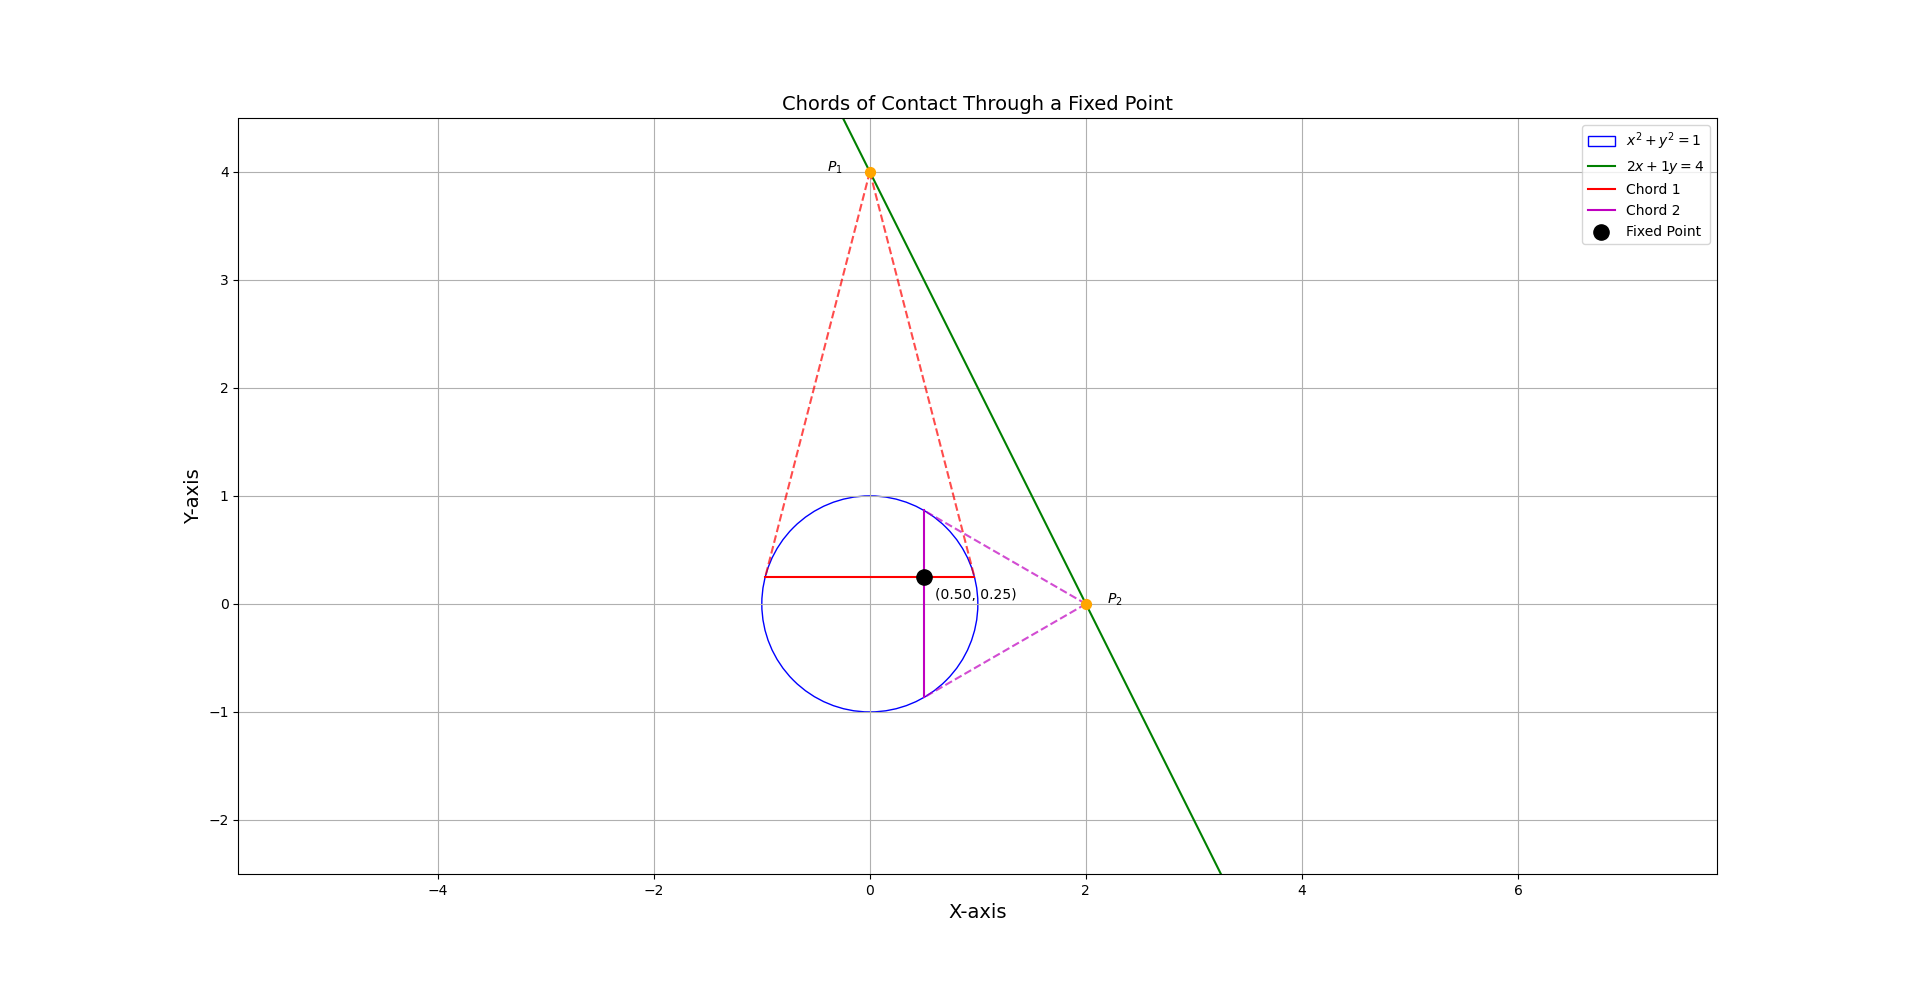
\includegraphics[width=0.7\columnwidth]{figs/fig1.png}
	\caption{}
   \label{}
\end{figure}
\end{frame}

\section{C Code}
\begin{frame}[fragile]
\frametitle{C Code}
\begin{lstlisting}[language=C]
 void get_circle_params(double* out_data) {
    out_data[0] = 0.0; 
    out_data[1] = 1.0; 
    out_data[2] = 1.0; 
}
    \end{lstlisting}
\end{frame}

\section{Python Code}
\begin{frame}[fragile]
\frametitle{Python Code for Solving}
\begin{lstlisting}[language=Python]
import ctypes
import sympy

def find_locus_equation():
     
    lib = ctypes.CDLL('./code.so')
   
    double_array_3 = ctypes.c_double * 3
    lib.get_circle_params.argtypes = [ctypes.POINTER(ctypes.c_double)]
    out_data_c = double_array_3()
    lib.get_circle_params(out_data_c)
     
    c1_x, c1_y, r1 = list(out_data_c)
    c1_center = (c1_x, c1_y)
 
    h, k = sympy.symbols('h k', real=True)
    r = sympy.Abs(k)
    lhs = (h - c1_center[0])**2 + (k - c1_center[1])**2

\end{lstlisting}
\end{frame}
\begin{frame}[fragile]
\frametitle{Python Code for Solving}
\begin{lstlisting}[language=Python]
   rhs = (r + r1)**2
    locus_eq = sympy.simplify(lhs - rhs)
    x, y = sympy.symbols('x y')
    final_locus = locus_eq.subs([(h, x), (k, y)])
    
    return sympy.Eq(final_locus, 0)
\end{lstlisting}
\end{frame}
\begin{frame}[fragile]
\frametitle{Python Code for Plotting}
\begin{lstlisting}[language=Python]
# Code by /sdcard/github/matgeo/codes/CoordGeoVV Sharma
# September 12, 2023
# Revised July 21, 2024
# Released under GNU GPL
# Section Formula
import sys
sys.path.insert(0, '/workspaces/urban-potato/matgeo/codes/CoordGeo/') 
import numpy as np
import matplotlib.pyplot as plt
from call import find_locus_equation  

locus_equation = find_locus_equation()
 
print(f"Locus equation: {locus_equation}")
fig, ax = plt.subplots(figsize=(8, 8))
  
c1 = plt.Circle((0, 1), 1, color='blue', fill=False, label='$x^2 + (y-1)^2 = 1$')

\end{lstlisting}
\end{frame}
\begin{frame}[fragile]
\frametitle{Python Code for Plotting}
\begin{lstlisting}[language=Python]
ax.add_patch(c1)
 
x_vals = np.linspace(-10, 10, 400)
y_vals = x_vals**2 / 4
ax.plot(x_vals, y_vals, 'r-', label=f'Locus: $x^2=4y$')
ax.plot([0, 0], [-10, 0], 'r-') 
ax.set_title("Locus of the Centre of the Touching Circle")
ax.set_xlabel("x"); ax.set_ylabel("y")
ax.grid(True); ax.axis('equal'); ax.legend()
plt.show()
plt.savefig('fig1.png')
\end{lstlisting}
\end{frame}
\end{document}
